\begin{frame}{有理数的大小比较规则}
\begin{block}{有理数大小比较法则}
\begin{enumerate}[label={\arabic*.}]
  \item 数轴上右边的数比左边的数\alert{大}
  \item 正数 \alert{>} 0
  \item 负数 \alert{<} 0
  \item 正数 \alert{>} 负数
  \item 两个负数比较,绝对值大的反而\alert{小}!
\end{enumerate}
\end{block}

\end{frame}

\begin{frame}{数轴比较法}
\begin{example}
  把下列各数表示在数轴上,并用"<"连接:\\
  $-2,\ 0,\ 3,\ -3.5,\ 1.5$
\end{example}

\pause
\begin{block}{解:}
\begin{enumerate}[label={\arabic*.}]
  \item 画数轴并标出所有数
  \begin{figure}
  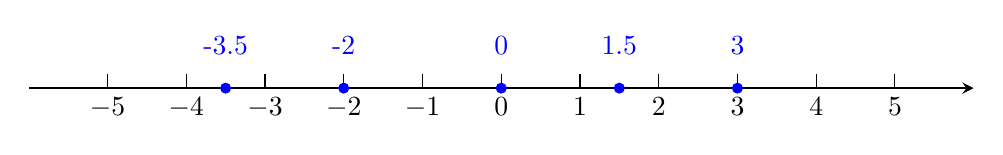
\begin{tikzpicture}
  \draw [black, thick, ->, >=stealth] (-6,0) -- (6,0); 
  \foreach \x in {-5, ..., 5}
  	\draw (\x cm,5pt) -- (\x cm,0pt) node[anchor=north] {$\x$};
  \foreach \x in {-2, 0, 3, -3.5, 1.5}
    \fill [blue] (\x,0) circle(2pt) node [above=0.3cm] {\x};
  \end{tikzpicture}
  \end{figure}
  \item 从左到右(从小到大)排列
  \item 结果:$-3.5 \alert{<} -2 \alert{<}  0 \alert{<}  1.5 \alert{<}  3$
\end{enumerate}
\end{block}
\end{frame}

\begin{frame}{两负数的绝对值比较法}
\textbf{两个负数比较,绝对值大的反而\alert{小}!}
\begin{example}
(1) -3 与 -5 哪个大? (2) -1.3 与 -3 哪个大?\\
\end{example}
\pause
\begin{block}{解:}
(1) \\
$| -3 | = 3, \quad | -5 | = 5, $ \\
$\because 3 < 5, $ \\
$\therefore -3 > -5$ \\
(2) \\
$| -1.3 | = 1.3, \quad |-3| = 3, $ \\
$\because 1.3 < 4, $\\
$\therefore -1.3 > -3$
\end{block}
\end{frame}